\documentclass[tikz,border=10pt]{standalone}
\usetikzlibrary{decorations.pathmorphing,patterns,arrows.meta,calc,positioning}
\usepackage{xcolor}

% --- Color Palette (Matching TesisPrincipal.tex) ----------------------
\definecolor{mnnwInk}     {HTML}{0A0A0A}
\definecolor{mnnwSignal}  {HTML}{0A84FF}
\definecolor{mnnwHair}    {HTML}{C9C9C9}
\definecolor{mnnwMute}    {HTML}{6F6F6F}
\definecolor{reticleFill} {HTML}{DCE6F7}  % light blue (reticle, j=1)
\definecolor{reticleEdge} {HTML}{4F6F9F}
\definecolor{reticleFlex} {HTML}{EEF3FB}  % flex couplings, lighter
\definecolor{waferFill}   {HTML}{F5DCDC}  % light red (wafer, j=3)
\definecolor{waferEdge}   {HTML}{9F4F4F}
\definecolor{waferFlex}   {HTML}{FBEEEE}
\definecolor{opticsFill}  {HTML}{E7DCF5}  % light purple (optics, j=2)
\definecolor{opticsEdge}  {HTML}{6F4F9F}
\definecolor{opticsFlex}  {HTML}{F3EEFB}
\definecolor{frameFill}   {HTML}{D9E8D2}  % light green (frames F1,F2)
\definecolor{frameEdge}   {HTML}{4F7F3F}
\definecolor{lensFill}    {HTML}{EEEEEE}

% --- Spring/damper definitions (from cap02.tex) -----------------------
\tikzset{
  hdamper/.pic={
    \draw[line width=0.5pt, mnnwInk] (-0.45,0)            -- (-0.18,0);
    \draw[line width=0.5pt, mnnwInk] (-0.18,-0.11) rectangle (0.18,0.11);
    \draw[line width=0.5pt, mnnwInk] (0,-0.11)            -- (0,0.11);
    \draw[line width=0.5pt, mnnwInk] (0.18,0)             -- (0.45,0);
  },
  vdamper/.pic={
    \draw[line width=0.5pt, mnnwInk] (0,-0.45)            -- (0,-0.18);
    \draw[line width=0.5pt, mnnwInk] (-0.11,-0.18) rectangle (0.11,0.18);
    \draw[line width=0.5pt, mnnwInk] (-0.11,0)            -- (0.11,0);
    \draw[line width=0.5pt, mnnwInk] (0,0.18)             -- (0,0.45);
  },
}

\newcommand{\hdamperLong}[3]{%
  \pgfmathsetmacro{\xa}{#1}\pgfmathsetmacro{\xb}{#2}\pgfmathsetmacro{\yy}{#3}
  \pgfmathsetmacro{\Lcyl}{(\xb-\xa)*0.55}
  \pgfmathsetmacro{\xcylR}{\xa+\Lcyl}
  \pgfmathsetmacro{\xpisR}{\xb}
  \draw[line width=0.5pt, mnnwInk] (\xa,\yy-0.13) -- (\xa,\yy+0.13);
  \draw[line width=0.5pt, mnnwInk] (\xa,\yy+0.13) -- (\xcylR,\yy+0.13);
  \draw[line width=0.5pt, mnnwInk] (\xa,\yy-0.13) -- (\xcylR,\yy-0.13);
  \pgfmathsetmacro{\xpiston}{\xa+\Lcyl*0.70}
  \draw[line width=0.5pt, mnnwInk] (\xpiston,\yy-0.11) -- (\xpiston,\yy+0.11);
  \draw[line width=0.5pt, mnnwInk] (\xpiston,\yy) -- (\xpisR,\yy);
}

% --- Chain Row Macro (from cap02.tex) ---------------------------------
\def\lastSpringY{-100}
\def\lastX{-100}
\def\getfirstchar#1#2\relax{#1}

\newcommand{\chainrow}[8]{%
  \edef\styleName{#2}\def\currColor{mnnwMute}
  \edef\firstChar{\expandafter\getfirstchar\styleName\relax}
  \if\firstChar w\def\currColor{waferEdge}\fi
  \if\firstChar o\def\currColor{opticsEdge}\fi
  \if\firstChar r\def\currColor{reticleEdge}\fi
  \pgfmathparse{abs(#3 - \lastX) < 0.001 ? 1 : 0}
  \ifnum\pgfmathresult=1
    \pgfmathparse{abs(#3) < 0.001 ? 1 : 0}
    \ifnum\pgfmathresult=1 \def\lineColor{frameEdge}\else \def\lineColor{\currColor}\fi
    \draw[line width=0.35pt, \lineColor] (#3, \lastSpringY) -- (#3, #1-0.62);
  \fi
  \node[#2, inner xsep=6pt] (blk) at (#4,#1) {#5};
  \node[ghost, inner xsep=6pt] at (#3,#1) {\phantom{#5}};
  \draw[hsp] (#3, #1+0.62) -- (#4, #1+0.62);
  \draw[line width=0.35pt, mnnwInk] (#3, #1+0.275) -- (#3, #1+0.62);
  \draw[line width=0.35pt, mnnwInk] (#4, #1+0.275) -- (#4, #1+0.62);
  \draw[line width=0.35pt, mnnwInk] (#3, #1-0.275) -- (#3, #1-0.62);
  \draw[line width=0.35pt, mnnwInk] (#4, #1-0.275) -- (#4, #1-0.62);
  \hdamperLong{#3}{#4}{#1-0.62}
  \pgfmathsetmacro{\lblAnch}{#4 > #3 ? "east" : "west"}
  \node[lbl, anchor=\lblAnch] at (#3, #1+0.62) {#6};
  \node[lbl, anchor=\lblAnch] at (#3, #1-0.62) {#7};
  \pgfmathsetmacro{\fAnch}{#4 > #3 ? "west" : "east"}
  \node[ftn, anchor=\fAnch] at (#4, #1-0.525) {#8};
  \draw[darr] (#3, #1-0.275) -- (#4, #1-0.275);
  \pgfmathsetmacro{\newSpringY}{#1+0.62}\xdef\lastSpringY{\newSpringY}
  \pgfmathsetmacro{\newX}{#4}\xdef\lastX{\newX}
}

\begin{document}
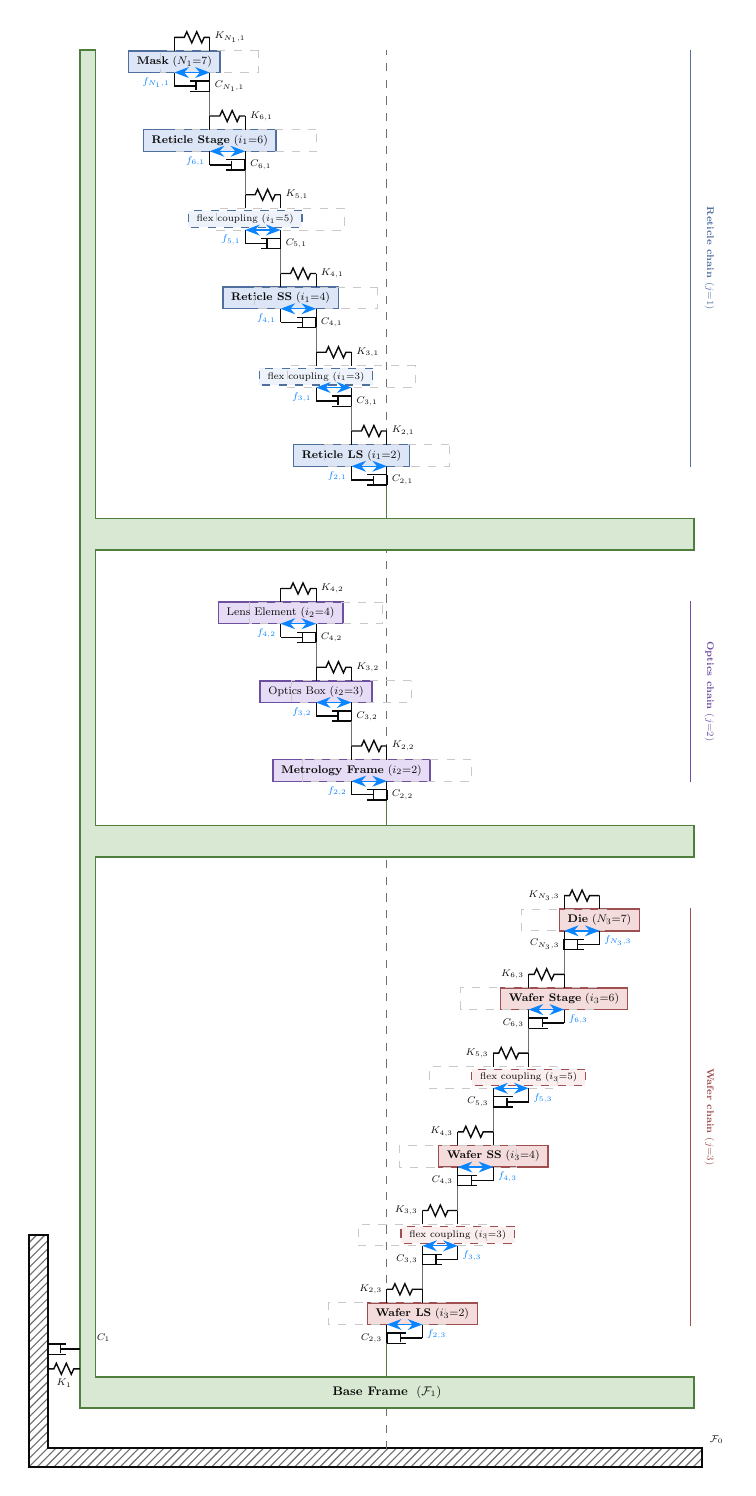
\begin{tikzpicture}[scale=0.5, transform shape,
  every node/.style    ={font=\small},
  rfrm/.style          ={draw=frameEdge, line width=0.6pt, fill=frameFill, minimum height=0.80cm, font=\small\bfseries, inner sep=2pt},
  rblk/.style          ={draw=reticleEdge, line width=0.5pt, fill=reticleFill, minimum height=0.55cm, font=\footnotesize, text=mnnwInk, inner sep=2.5pt},
  rflx/.style          ={draw=reticleEdge, line width=0.4pt, fill=reticleFlex, minimum height=0.42cm, font=\scriptsize, text=mnnwInk, inner sep=2pt, dashed},
  wblk/.style          ={draw=waferEdge, line width=0.5pt, fill=waferFill, minimum height=0.55cm, font=\footnotesize, text=mnnwInk, inner sep=2.5pt},
  wflx/.style          ={draw=waferEdge, line width=0.4pt, fill=waferFlex, minimum height=0.42cm, font=\scriptsize, text=mnnwInk, inner sep=2pt, dashed},
  oblk/.style          ={draw=opticsEdge, line width=0.5pt, fill=opticsFill, minimum height=0.55cm, font=\footnotesize, text=mnnwInk, inner sep=2.5pt},
  oflx/.style          ={draw=opticsEdge, line width=0.4pt, fill=opticsFlex, minimum height=0.42cm, font=\scriptsize, text=mnnwInk, inner sep=2pt, dashed},
  ghost/.style         ={draw=mnnwHair, dashed, line width=0.35pt, fill=none, minimum height=0.55cm},
  hsp/.style           ={line width=0.5pt, mnnwInk, decorate, decoration={zigzag, segment length=3.6pt, amplitude=2pt, pre length=2pt, post length=2pt}},
  vsp/.style           ={line width=0.5pt, mnnwInk, decorate, decoration={zigzag, segment length=3.6pt, amplitude=2pt, pre length=2pt, post length=2pt}},
  darr/.style          ={Stealth-Stealth, line width=0.5pt, mnnwSignal},
  lbl/.style           ={font=\scriptsize, text=mnnwInk},
  ftn/.style           ={font=\scriptsize, text=mnnwSignal},
  axis/.style          ={dashed, line width=0.4pt, mnnwMute},
  pillar/.style        ={fill=black!8, draw=mnnwHair, line width=0.3pt},
  hatchfloor/.style    ={pattern=north east lines, pattern color=mnnwMute},
]

\def\xLeft{-8.0}\def\xRight{8.0}\def\xPilR{7.4}
\def\yFloor{0}\def\yBase{1.4}
\def\yWa{3.4}\def\yWb{5.4}\def\yWc{7.4}\def\yWd{9.4}\def\yWe{11.4}\def\yWf{13.4}
\def\yOa{17.2}\def\yOb{19.2}\def\yOc{21.2}
\def\yRa{25.2}\def\yRb{27.2}\def\yRc{29.2}\def\yRd{31.2}\def\yRe{33.2}\def\yRf{35.2}
\def\yTop{35.5}\def\yShA{15.4}\def\yShB{23.2}

\filldraw[hatchfloor, draw=mnnwInk, line width=0.7pt]
  (\xRight, 0) -- (\xLeft-0.6, 0) -- (\xLeft-0.6, \yWb) -- (\xLeft-1.1, \yWb) 
  -- (\xLeft-1.1, -0.5) -- (\xRight, -0.5) -- cycle;
\node[lbl, anchor=west] at (\xRight+0.08,0.20) {$\mathcal{F}_0$};
\draw[axis] (0,-0.05) -- (0,\yTop);

\filldraw[draw=frameEdge, line width=0.6pt, fill=frameFill]
  (7.8, \yBase-0.4) -- (-7.8, \yBase-0.4) -- (-7.8, \yTop) -- (-7.4, \yTop)
  -- (-7.4, \yShB+0.4) -- (7.8, \yShB+0.4) -- (7.8, \yShB-0.4) -- (-7.4, \yShB-0.4)
  -- (-7.4, \yShA+0.4) -- (7.8, \yShA+0.4) -- (7.8, \yShA-0.4) -- (-7.4, \yShA-0.4)
  -- (-7.4, \yBase+0.4) -- (7.8, \yBase+0.4) -- cycle;
\node[font=\small\bfseries, text=mnnwInk] at (0, \yBase) {Base Frame $\;(\mathcal{F}_1)$};

\hdamperLong{\xLeft-0.6}{-7.8}{2.5}
\node[lbl, above=2pt] at (-7.2, 2.5) {$C_1$};
\draw[hsp] (\xLeft-0.6, 2.0) -- (-7.8, 2.0) node[midway, below=4pt, lbl] {$K_1$};

\pgfmathsetmacro{\shelfW}{\yBase+0.4}
\xdef\lastSpringY{\shelfW} \xdef\lastX{0}
\chainrow{\yWa}{wblk}{0}{ 0.9}{\textbf{Wafer LS} $(i_3{=}2)$}{$K_{2,3}$}{$C_{2,3}$}{$f_{2,3}$}
\chainrow{\yWb}{wflx}{0.9}{ 1.8}{flex coupling $(i_3{=}3)$}{$K_{3,3}$}{$C_{3,3}$}{$f_{3,3}$}
\chainrow{\yWc}{wblk}{1.8}{ 2.7}{\textbf{Wafer SS} $(i_3{=}4)$}{$K_{4,3}$}{$C_{4,3}$}{$f_{4,3}$}
\chainrow{\yWd}{wflx}{2.7}{ 3.6}{flex coupling $(i_3{=}5)$}{$K_{5,3}$}{$C_{5,3}$}{$f_{5,3}$}
\chainrow{\yWe}{wblk}{3.6}{ 4.5}{\textbf{Wafer Stage} $(i_3{=}6)$}{$K_{6,3}$}{$C_{6,3}$}{$f_{6,3}$}
\chainrow{\yWf}{wblk}{4.5}{ 5.4}{\textbf{Die} $(N_3{=}7)$}{$K_{N_3,3}$}{$C_{N_3,3}$}{$f_{N_3,3}$}

\pgfmathsetmacro{\shelfO}{\yShA+0.4}
\xdef\lastSpringY{\shelfO} \xdef\lastX{0}
\chainrow{\yOa}{oblk}{0}{-0.9}{\textbf{Metrology Frame} $(i_2{=}2)$}{$K_{2,2}$}{$C_{2,2}$}{$f_{2,2}$}
\chainrow{\yOb}{oblk}{-0.9}{-1.8}{Optics Box $(i_2{=}3)$}{$K_{3,2}$}{$C_{3,2}$}{$f_{3,2}$}
\chainrow{\yOc}{oblk}{-1.8}{-2.7}{Lens Element $(i_2{=}4)$}{$K_{4,2}$}{$C_{4,2}$}{$f_{4,2}$}

\pgfmathsetmacro{\shelfR}{\yShB+0.4}
\xdef\lastSpringY{\shelfR} \xdef\lastX{0}
\chainrow{\yRa}{rblk}{0}{-0.9}{\textbf{Reticle LS} $(i_1{=}2)$}{$K_{2,1}$}{$C_{2,1}$}{$f_{2,1}$}
\chainrow{\yRb}{rflx}{-0.9}{-1.8}{flex coupling $(i_1{=}3)$}{$K_{3,1}$}{$C_{3,1}$}{$f_{3,1}$}
\chainrow{\yRc}{rblk}{-1.8}{-2.7}{\textbf{Reticle SS} $(i_1{=}4)$}{$K_{4,1}$}{$C_{4,1}$}{$f_{4,1}$}
\chainrow{\yRd}{rflx}{-2.7}{-3.6}{flex coupling $(i_1{=}5)$}{$K_{5,1}$}{$C_{5,1}$}{$f_{5,1}$}
\chainrow{\yRe}{rblk}{-3.6}{-4.5}{\textbf{Reticle Stage} $(i_1{=}6)$}{$K_{6,1}$}{$C_{6,1}$}{$f_{6,1}$}
\chainrow{\yRf}{rblk}{-4.5}{-5.4}{\textbf{Mask} $(N_1{=}7)$}{$K_{N_1,1}$}{$C_{N_1,1}$}{$f_{N_1,1}$}

\draw[line width=0.4pt, waferEdge]   (\xPilR+0.30,\yWa-0.30) -- (\xPilR+0.30,\yWf+0.30);
\node[font=\scriptsize\bfseries, text=waferEdge, rotate=-90, anchor=south] at (\xPilR+0.55,{(\yWa+\yWf)/2}) {Wafer chain $(j{=}3)$};
\draw[line width=0.4pt, opticsEdge]  (\xPilR+0.30,\yOa-0.30) -- (\xPilR+0.30,\yOc+0.30);
\node[font=\scriptsize\bfseries, text=opticsEdge, rotate=-90, anchor=south] at (\xPilR+0.55,{(\yOa+\yOc)/2}) {Optics chain $(j{=}2)$};
\draw[line width=0.4pt, reticleEdge] (\xPilR+0.30,\yRa-0.30) -- (\xPilR+0.30,\yRf+0.30);
\node[font=\scriptsize\bfseries, text=reticleEdge, rotate=-90, anchor=south] at (\xPilR+0.55,{(\yRa+\yRf)/2}) {Reticle chain $(j{=}1)$};

\end{tikzpicture}
\end{document}
